% \section{Cơ sở lý thuyết và công nghệ}
% \subsection{Cơ sở lý thuyết}
% \subsection{Công nghệ}
\section{Nghiên cứu thị trường}
% Tìm hiều về các hệ thống phần mềm tương tự hiện đang có trên thị trường
% Điểm yếu, điểm mạnh -> mục tiêu phát triển phần mềm của mình như thế nào

Hiện nay, trên thị trường quốc tế xuất hiện rất nhiều hệ thống chatbot và các nền tảng hỗ trợ chatbot tư vấn khách hàng. Tuy nhiên, trong phạm vi nghiên cứu này, nhóm tác giả sẽ tập trung phân tích một số hệ thống nổi bật tại thị trường Việt Nam. Mỗi hệ thống đều có những ưu điểm và hạn chế riêng, đi kèm với giao diện thân thiện và bộ tính năng đa dạng, phục vụ cho các nhu cầu khác nhau của doanh nghiệp.
\subsection{AhaChat}
\subsubsection{Giới thiệu}
AhaChat là một nền tảng tạo chatbot phổ biến tại Việt Nam, được thiết kế để hỗ trợ doanh nghiệp tự động hóa quy trình chăm sóc khách hàng và bán hàng qua các kênh như Facebook Messenger, Zalo và Instagram. Với giao diện trực quan và khả năng tạo chatbot không cần lập trình, AhaChat giúp doanh nghiệp dễ dàng thiết lập các kịch bản trò chuyện tự động, từ việc tư vấn sản phẩm, xử lý đơn hàng, đến chăm sóc khách hàng sau bán.

AhaChat được phát triển để giải quyết những thách thức mà nhiều doanh nghiệp gặp phải trong việc duy trì kết nối nhanh chóng và liên tục với khách hàng, đặc biệt qua các nền tảng mạng xã hội như Facebook và Zalo. Nhu cầu tự động hóa các tác vụ như trả lời tin nhắn, xử lý đơn hàng và chăm sóc khách hàng ngày càng trở nên cấp thiết khi số lượng người dùng trực tuyến tăng mạnh. AhaChat ra đời với sứ mệnh hỗ trợ doanh nghiệp giải quyết những vấn đề này thông qua chatbot, giúp tiết kiệm thời gian, chi phí, và tăng cường hiệu quả trong giao tiếp.

\href{https://ahachat.com/}{Link truy cập}
\subsubsection{UI/UX}
\begin{figure}[H]
    \centering
    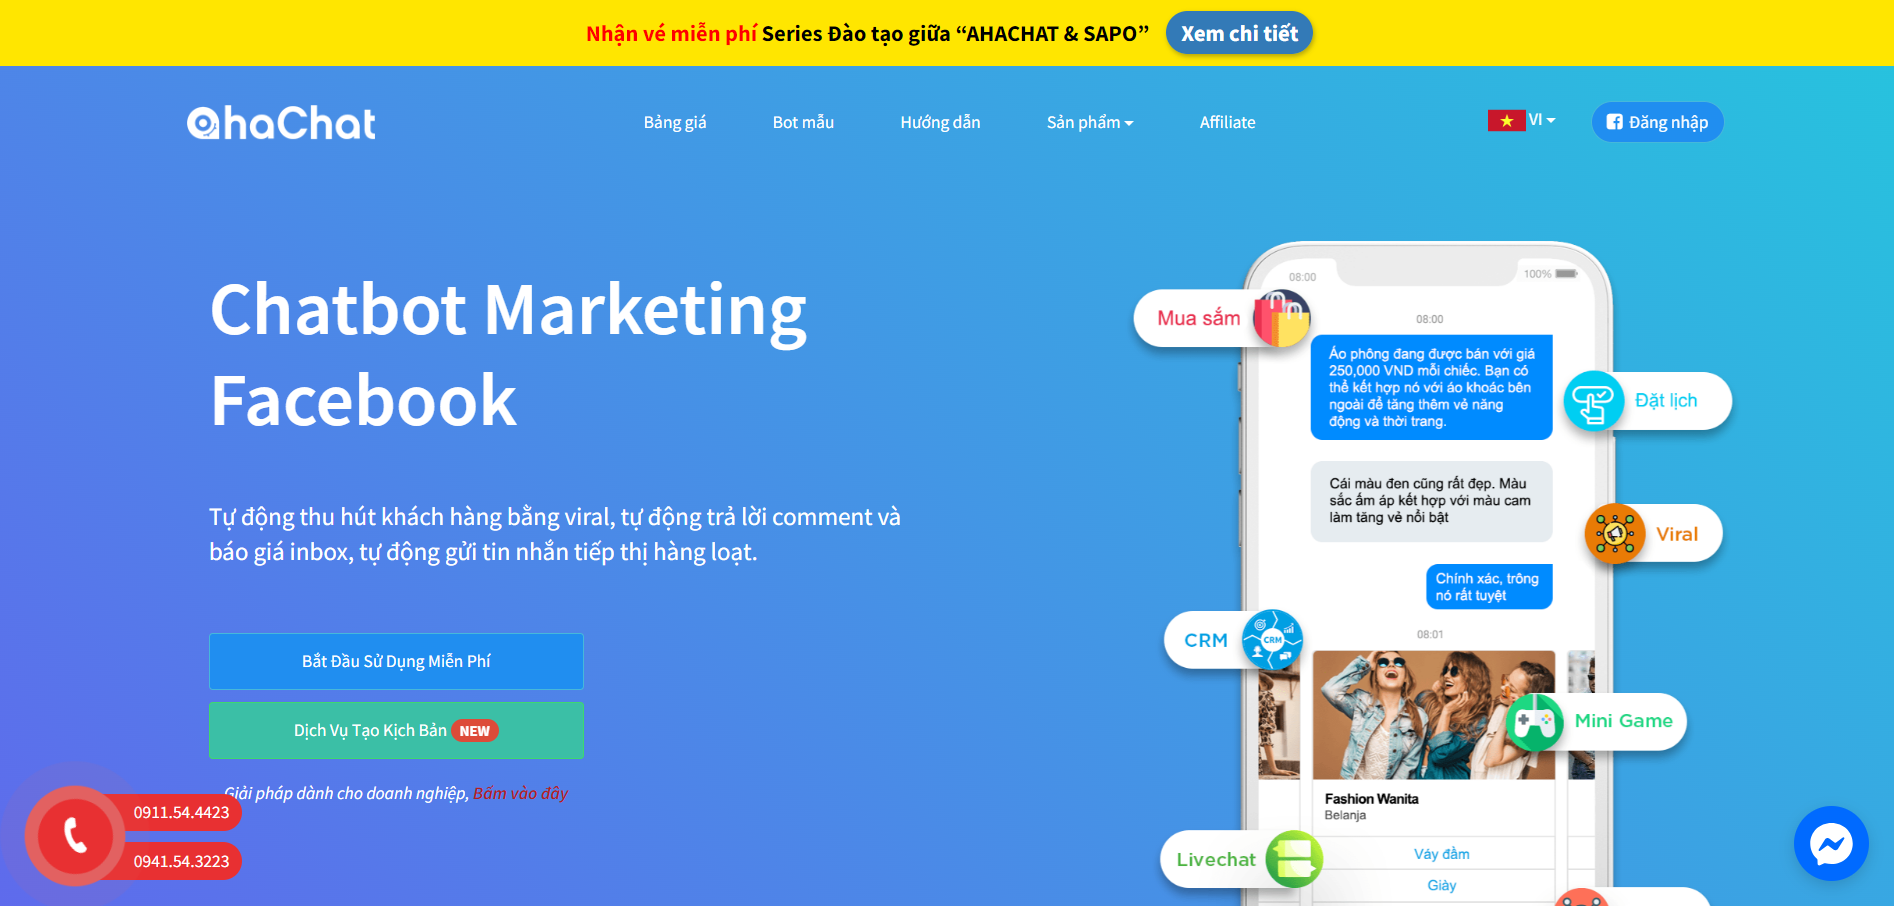
\includegraphics[width=1\linewidth]{Images/ahachatlanding.png}
    \vspace{0.5cm}
    \caption{Giao diện trang Landing page của AhaChat}
    \label{fig:enter-label}
\end{figure}
\begin{figure}[H]
    \centering
    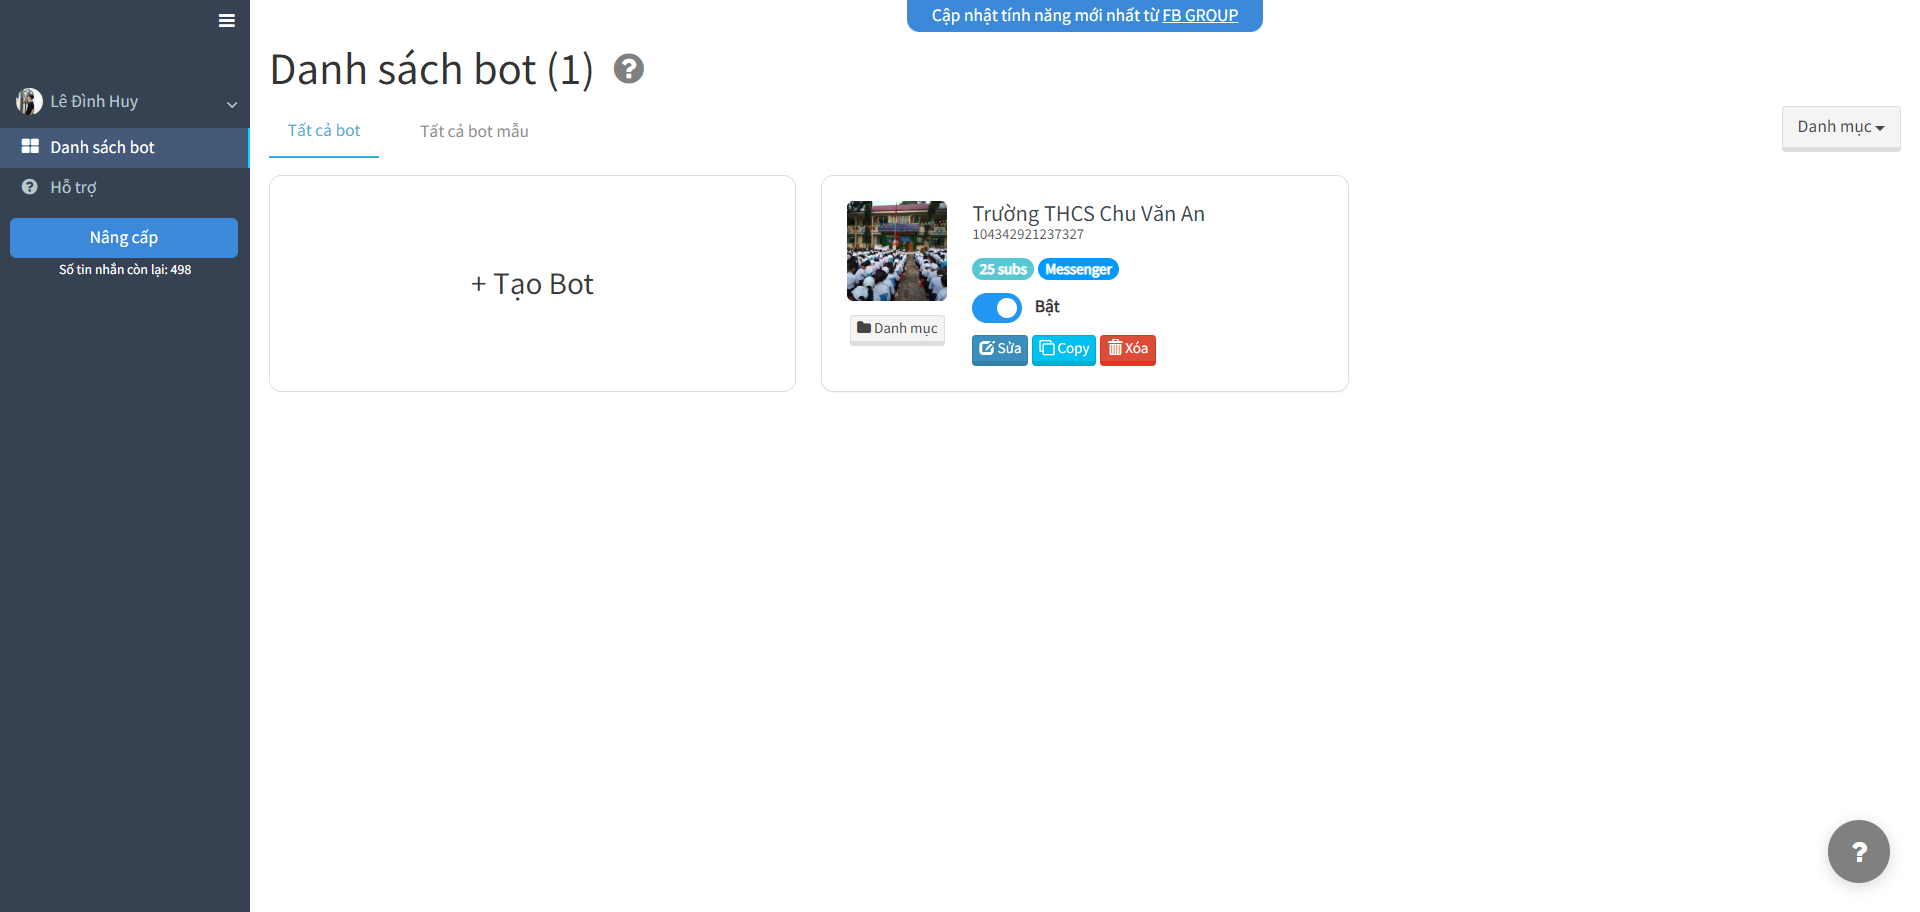
\includegraphics[width=1\linewidth]{Images/homeahachat.png}
    \vspace{0.5cm}
    \caption{Giao diện trang chủ của AhaChat}
    \label{fig:enter-label}
\end{figure}
\begin{figure}[H]
    \centering
    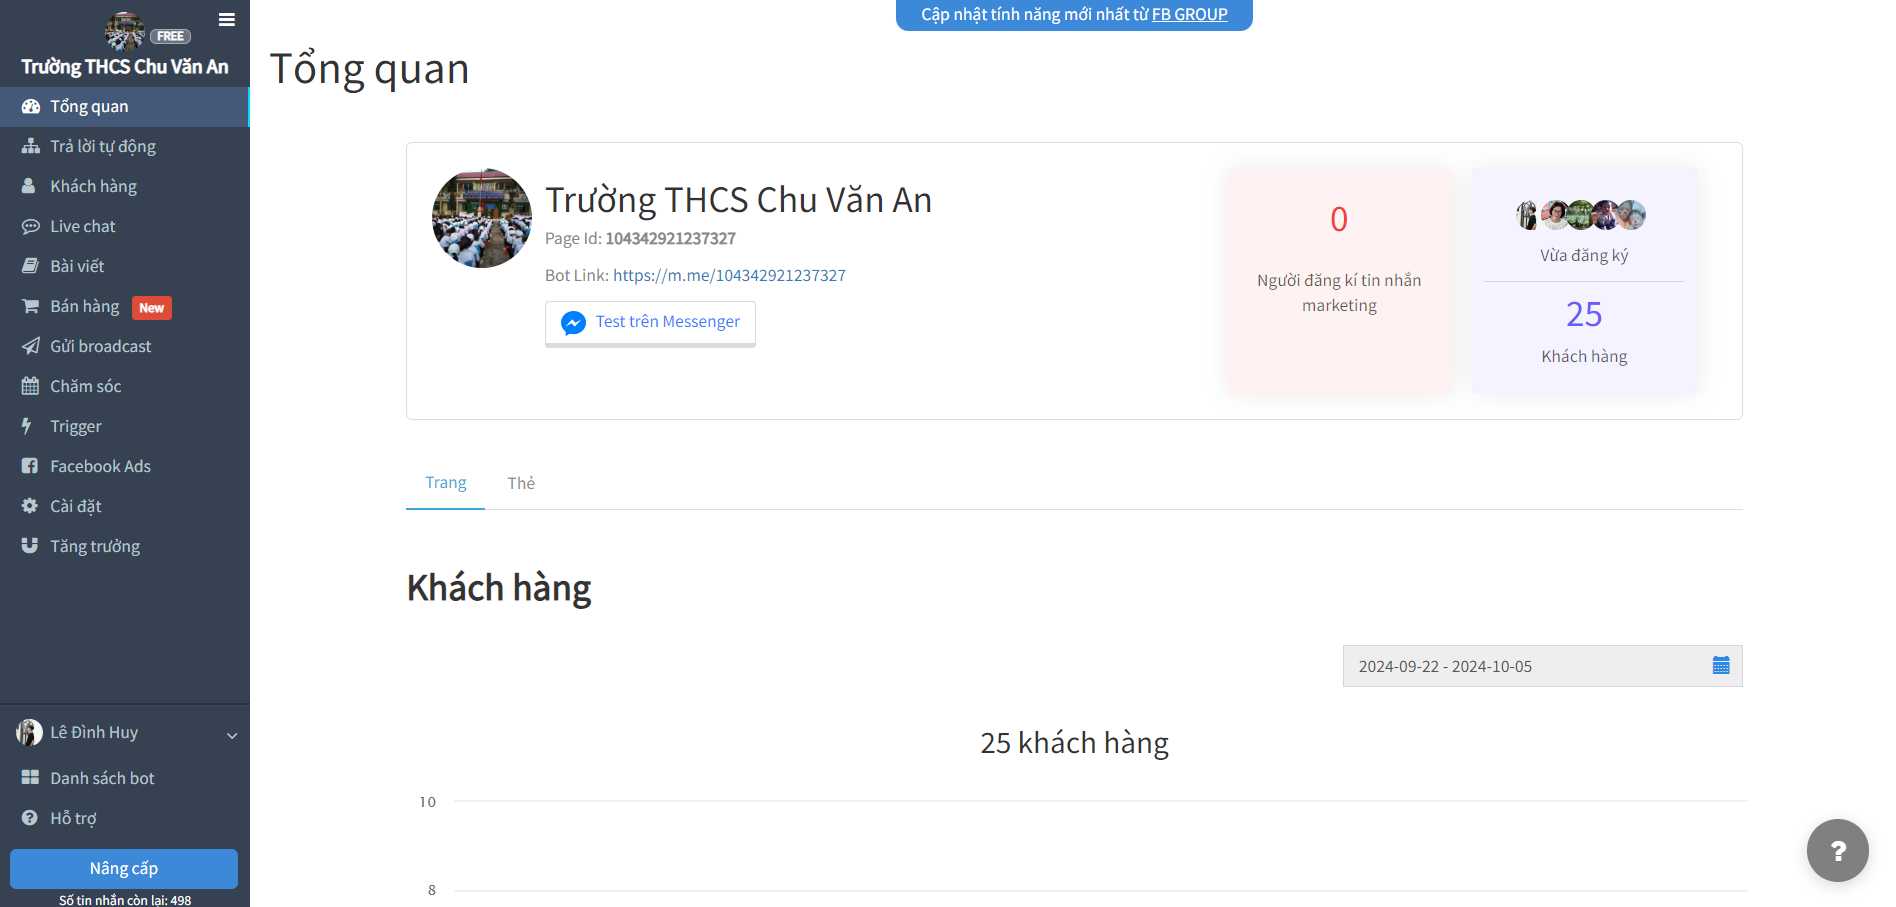
\includegraphics[width=1\linewidth]{Images/quanlypageahachat.png}
    \vspace{0.5cm}
    \caption{Giao diện quản lý fanpage Facebook của AhaChat}
    \label{fig:enter-label}
\end{figure}
\begin{figure}[H]
    \centering
    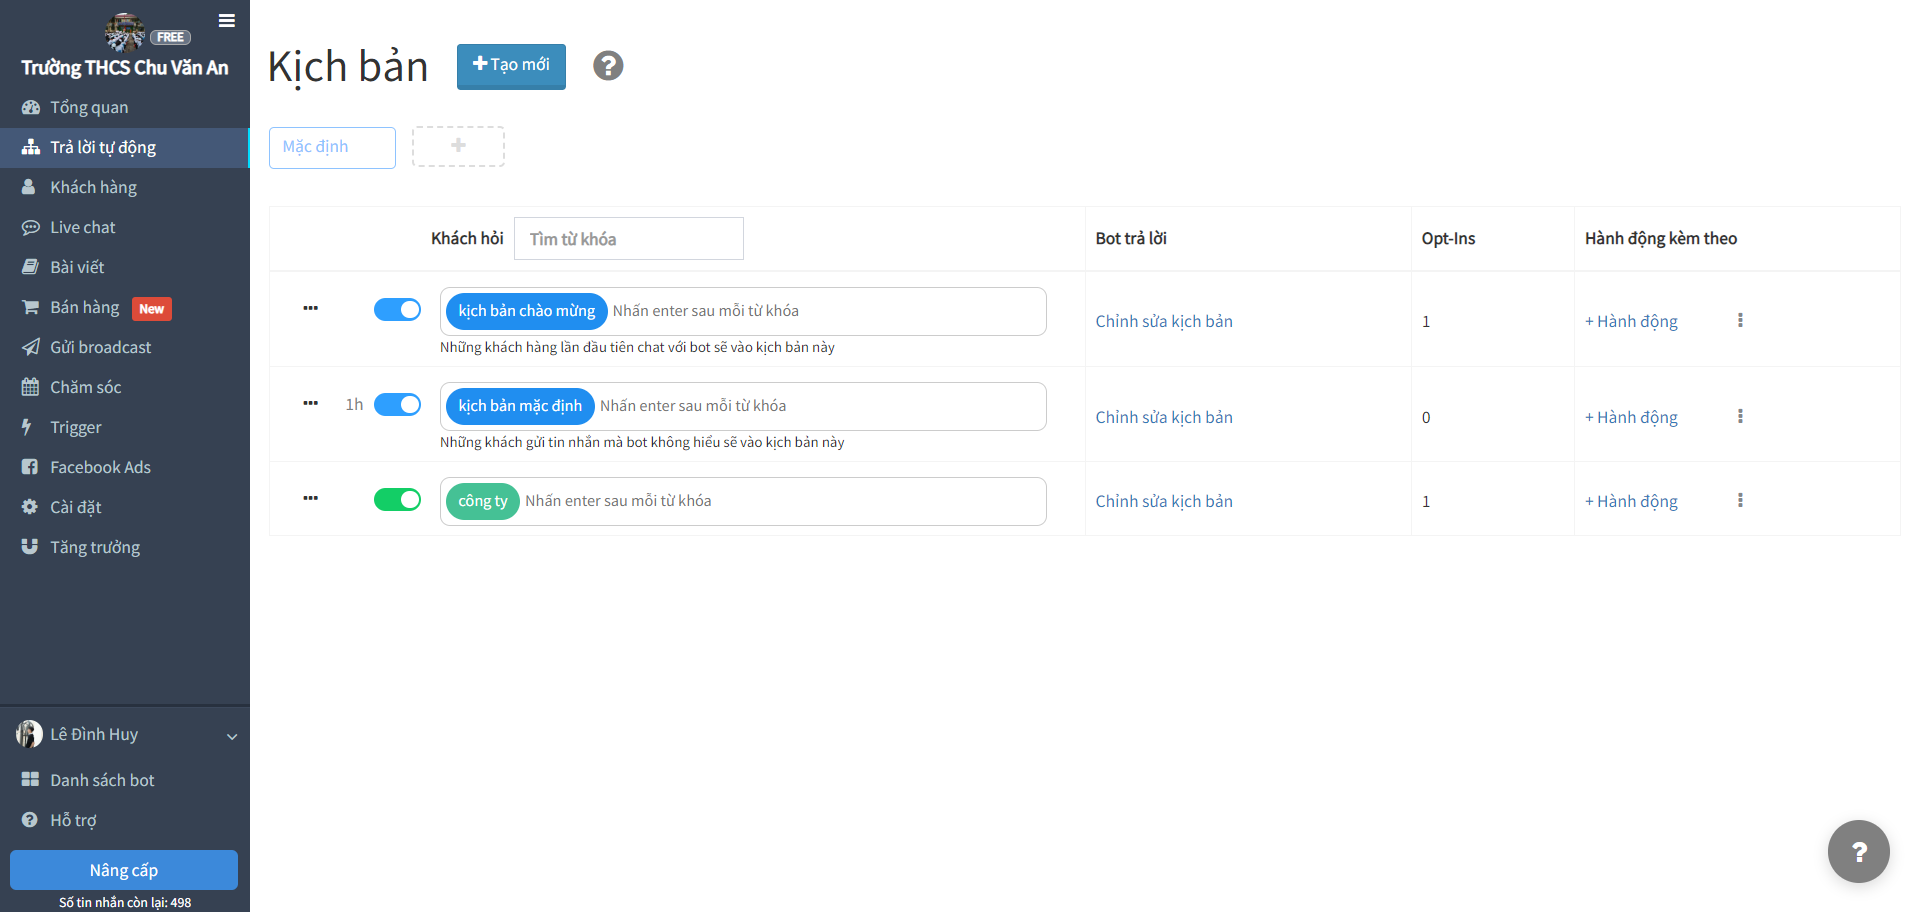
\includegraphics[width=1\linewidth]{Images/quanlykichbanahachat.png}
    \vspace{0.5cm}
    \caption{Giao diện quản lý kịch bản của AhaChat}
    \label{fig:enter-label}
\end{figure}
\subsubsection{Các tính năng chính}
AhaChat là một trong những nền tảng chatbot nổi bật tại Việt Nam, giúp doanh nghiệp tự động hóa giao tiếp và chăm sóc khách hàng hiệu quả. Dưới đây là các tính năng nổi bật giúp tối ưu quy trình bán hàng và tương tác khách hàng trên nhiều kênh trực tuyến.
\begin{itemize}
    \item \textbf{Tạo kịch bản trả lời tự động rất dễ bằng Mind Map:} Người dùng có thể xây dựng kịch bản chatbot một cách trực quan bằng sơ đồ tư duy, giúp dễ dàng tạo ra các cuộc hội thoại logic và hiệu quả.


\item \textbf{Lưu và lấy dữ liệu từ Google Sheets khôi lo sốt đơn:} Tích hợp Google Sheets giúp doanh nghiệp quản lý và theo dõi đơn hàng dễ dàng, không bỏ sót bất kỳ yêu cầu nào từ khách hàng.

\item \textbf{Nhân viên có thể chat trực tiếp với khách thông qua Live Chat:} Tính năng Live Chat cho phép nhân viên chăm sóc khách hàng giao tiếp trực tiếp với khách qua chatbot, tăng cường trải nghiệm khách hàng.

\item \textbf{Phân loại và gửi broadcast hàng loạt để Remarketing:} Doanh nghiệp có thể phân loại khách hàng và gửi tin nhắn hàng loạt cho các chiến dịch tiếp thị lại, giúp thu hút khách hàng tiềm năng quay trở lại.

\item \textbf{Đưa khách hàng vào phễu bằng chiến dịch Chăm sóc:} Quản lý khách hàng theo phễu tiếp thị và chăm sóc tự động, giúp duy trì mối quan hệ lâu dài với khách hàng.

\item \textbf{Auto Inbox để trả lời hàng ngàn comment cùng một lúc:} Chức năng tự động gửi tin nhắn trả lời vào hộp thư của hàng ngàn khách hàng cùng lúc, tiết kiệm thời gian quản lý tương tác.

\item \textbf{Dễ dàng bùng nổ đơn hàng bằng Chatbot Viral:} Sử dụng tính năng chatbot để lan truyền nhanh chóng các thông tin về sản phẩm/dịch vụ, thúc đẩy sự tăng trưởng doanh số.

\item \textbf{Xem thống kê khách hàng và tin nhắn theo thời gian thực:} Công cụ phân tích cho phép theo dõi và báo cáo khách hàng, tình hình tương tác và hiệu suất của chatbot trong thời gian thực.

\item \textbf{Có nhiều công cụ triển khai để tiếp cận khách hàng:} AhaChat cung cấp các công cụ đa dạng giúp doanh nghiệp dễ dàng triển khai các chiến lược tiếp cận và thu hút khách hàng hiệu quả hơn.
\end{itemize}
\begin{figure}[H]
    \centering
    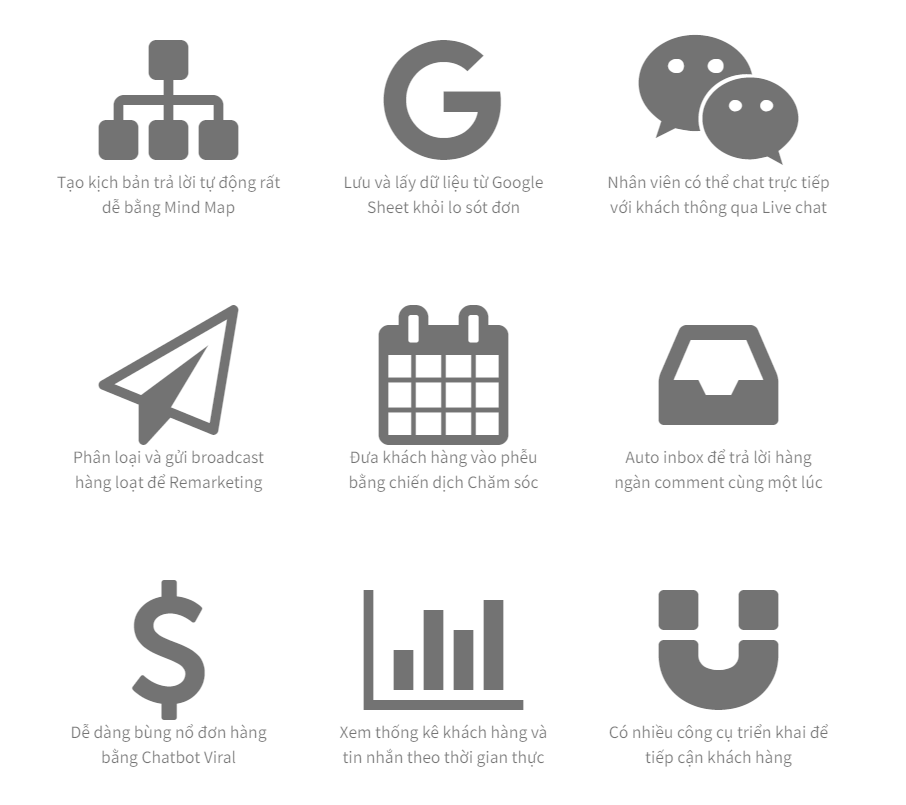
\includegraphics[width=0.75\linewidth]{Images/tinhnangahachat.png}
    \vspace{0.5cm}
    \caption{Giao diện quản lý kịch bản của AhaChat}
    \label{fig:enter-label}
\end{figure}
\subsubsection{Phân tích SWOT}
\begin{table}[H]
\centering
\begin{tabular}{|p{7cm}|p{7cm}|}
\hline
 \begin{center}
     Strengths
 \end{center} & \begin{center}
     Weaknesses
 \end{center}  \\
\hline
\begin{itemize}
    \item Giao diện dễ sử dụng với tính năng kéo-thả Mind Map.
    \item Hỗ trợ tích hợp đa kênh (Facebook,  Messenger, Zalo, Instagram).
    \item Tích hợp công cụ CRM giúp quản lý thông tin khách hàng hiệu quả.
    \item Tính năng tự động hóa quy trình bán hàng và chăm sóc khách hàng mạnh mẽ.
    \item Nhiều công cụ marketing như broadcast, remarketing, và chăm sóc tự động.
\end{itemize} &  
\begin{itemize}
    \item Chỉ tập trung chủ yếu vào thị trường Việt Nam và chưa hỗ trợ chatbot trên website.
\item Khả năng tùy chỉnh nâng cao có thể không đa dạng so với các nền tảng chatbot cao cấp hơn.
\end{itemize}\\
\hline
\begin{center}
    Opportunities
\end{center} & \begin{center}
    Threats
\end{center}\\
\hline
\begin{itemize}
    \item Nhu cầu ngày càng tăng về tự động hóa trong chăm sóc khách hàng và bán hàng trực tuyến tại Việt Nam.
    \item Tiềm năng mở rộng tích hợp với các hệ thống thanh toán, vận chuyển quốc tế.
\end{itemize} &  
\begin{itemize}
    \item Cạnh tranh gay gắt từ các nền tảng mạnh khác ở Việt Nam cũng như quốc tế.
    \item Tốc độ phát triển của công nghệ AI nhanh chóng, yêu cầu cải tiến liên tục để duy trì sự cạnh tranh.
\end{itemize}\\
\hline
\end{tabular}
\caption{Bảng phân tích SWOT cho hệ thống AhaChat}
\end{table}
\subsection{Fchat}
\subsubsection{Giới thiệu}
Fchat phát triển bởi Công ty Cổ phần SaleMall (SaleMall JSC) - đơn vị chuyên về các phần mềm quản lý bán hàng, chăm sóc khách hàng và hệ thống marketing. SaleMall nằm trong hệ sinh thái của Inet Group - tập đoàn hơn 18 năm hoạt động với hệ sinh thái đa dạng về công nghệ thông tin từ tên miền, hosting, VAT, website, đào tạo trực tuyến...

Theo đại diện SaleMall, cùng với sự phát triển mạnh mẽ của thương mại điện tử Việt Nam trong những năm gần đây, doanh nghiệp bán hàng luôn tìm kiếm giải pháp giao tiếp hiệu quả trên các nền tảng mạng xã hội, sàn thương mại điện tử, website... Công nghệ mang lại những cơ hội mới nhưng cũng ra tạo thách thức với chủ kinh doanh nếu không cập nhật kịp thời.

Để giải quyết khó khăn của những nhà bán hàng, Fchat mang đến giải pháp chăm sóc khách hàng hiệu quả hơn. Phần mềm chatbot có khả năng tự động trả lời câu hỏi 24/7, hỗ trợ trả lời tin nhắn và chăm sóc hàng nghìn người cùng một lúc mà không bị gián đoạn. Điều này giúp Fchat trở thành công cụ hỗ trợ hiệu quả cho doanh nghiệp kinh doanh online.

\href{https://fchat.vn/}{Link truy cập}
\subsubsection{UI/UX}
\begin{figure}[H]
    \centering
    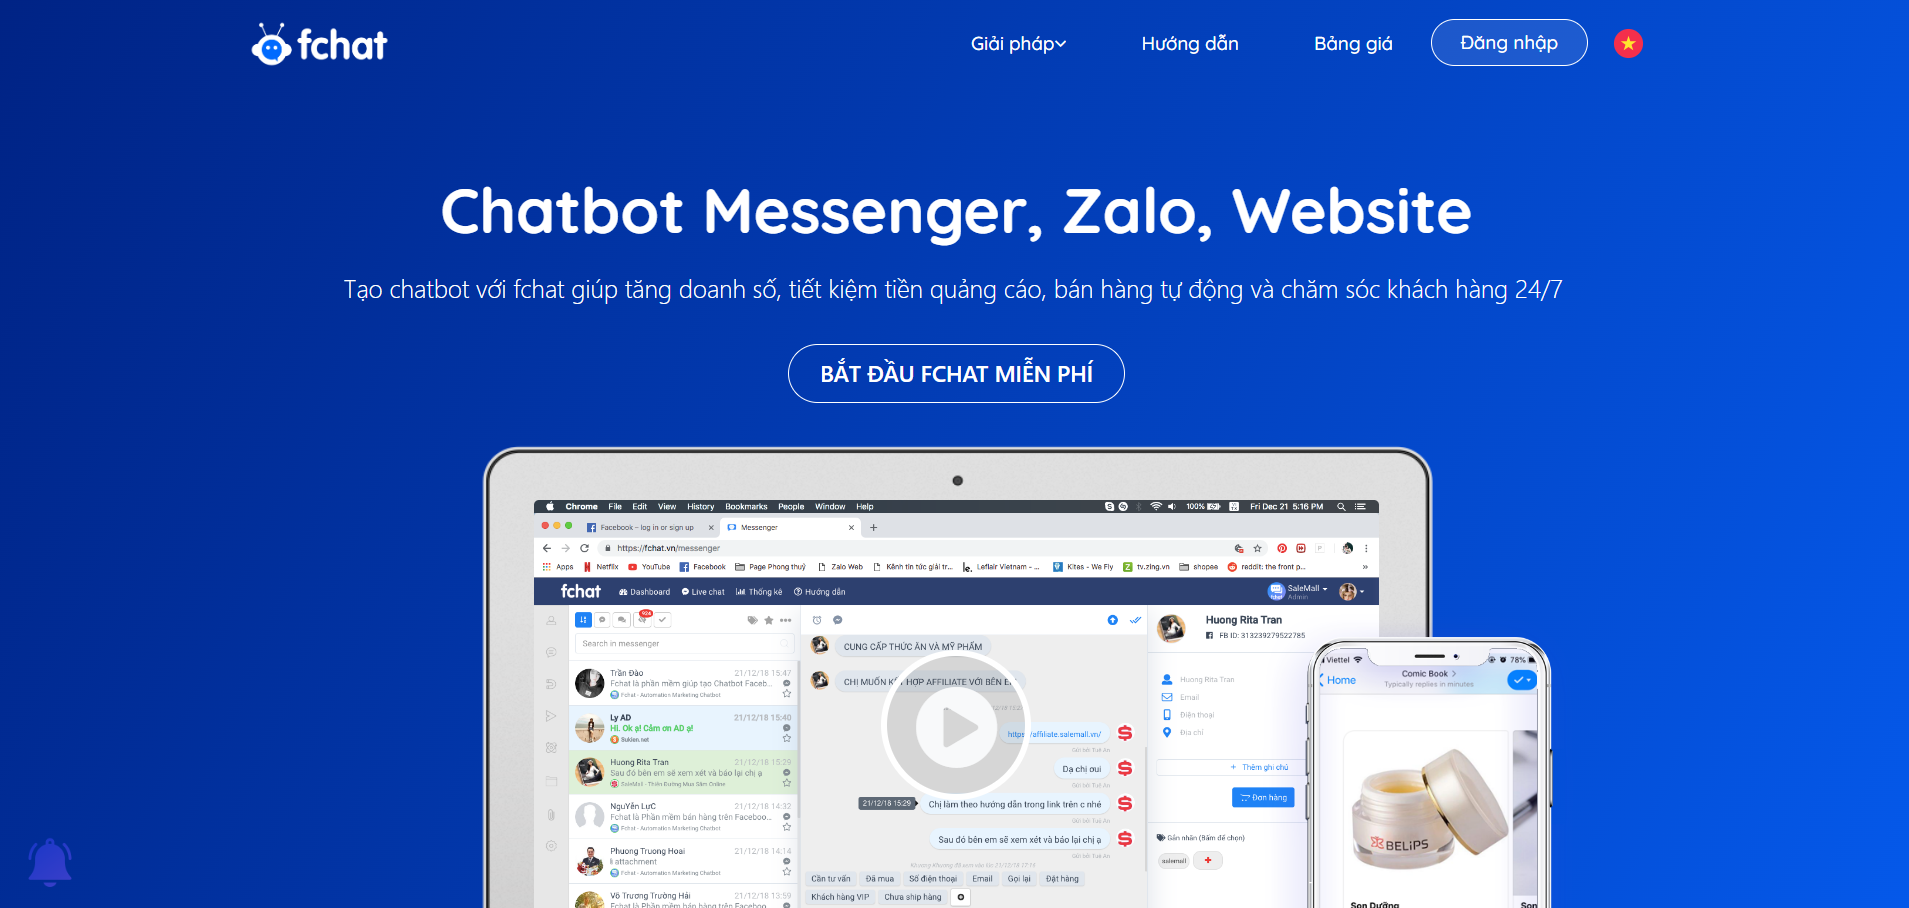
\includegraphics[width=1\linewidth]{Images/landingfchat.png}
    \vspace{0.5cm}
    \caption{Giao diện trang Landing page của Fchat}
    \label{fig:enter-label}
\end{figure}
\begin{figure}[H]
    \centering
    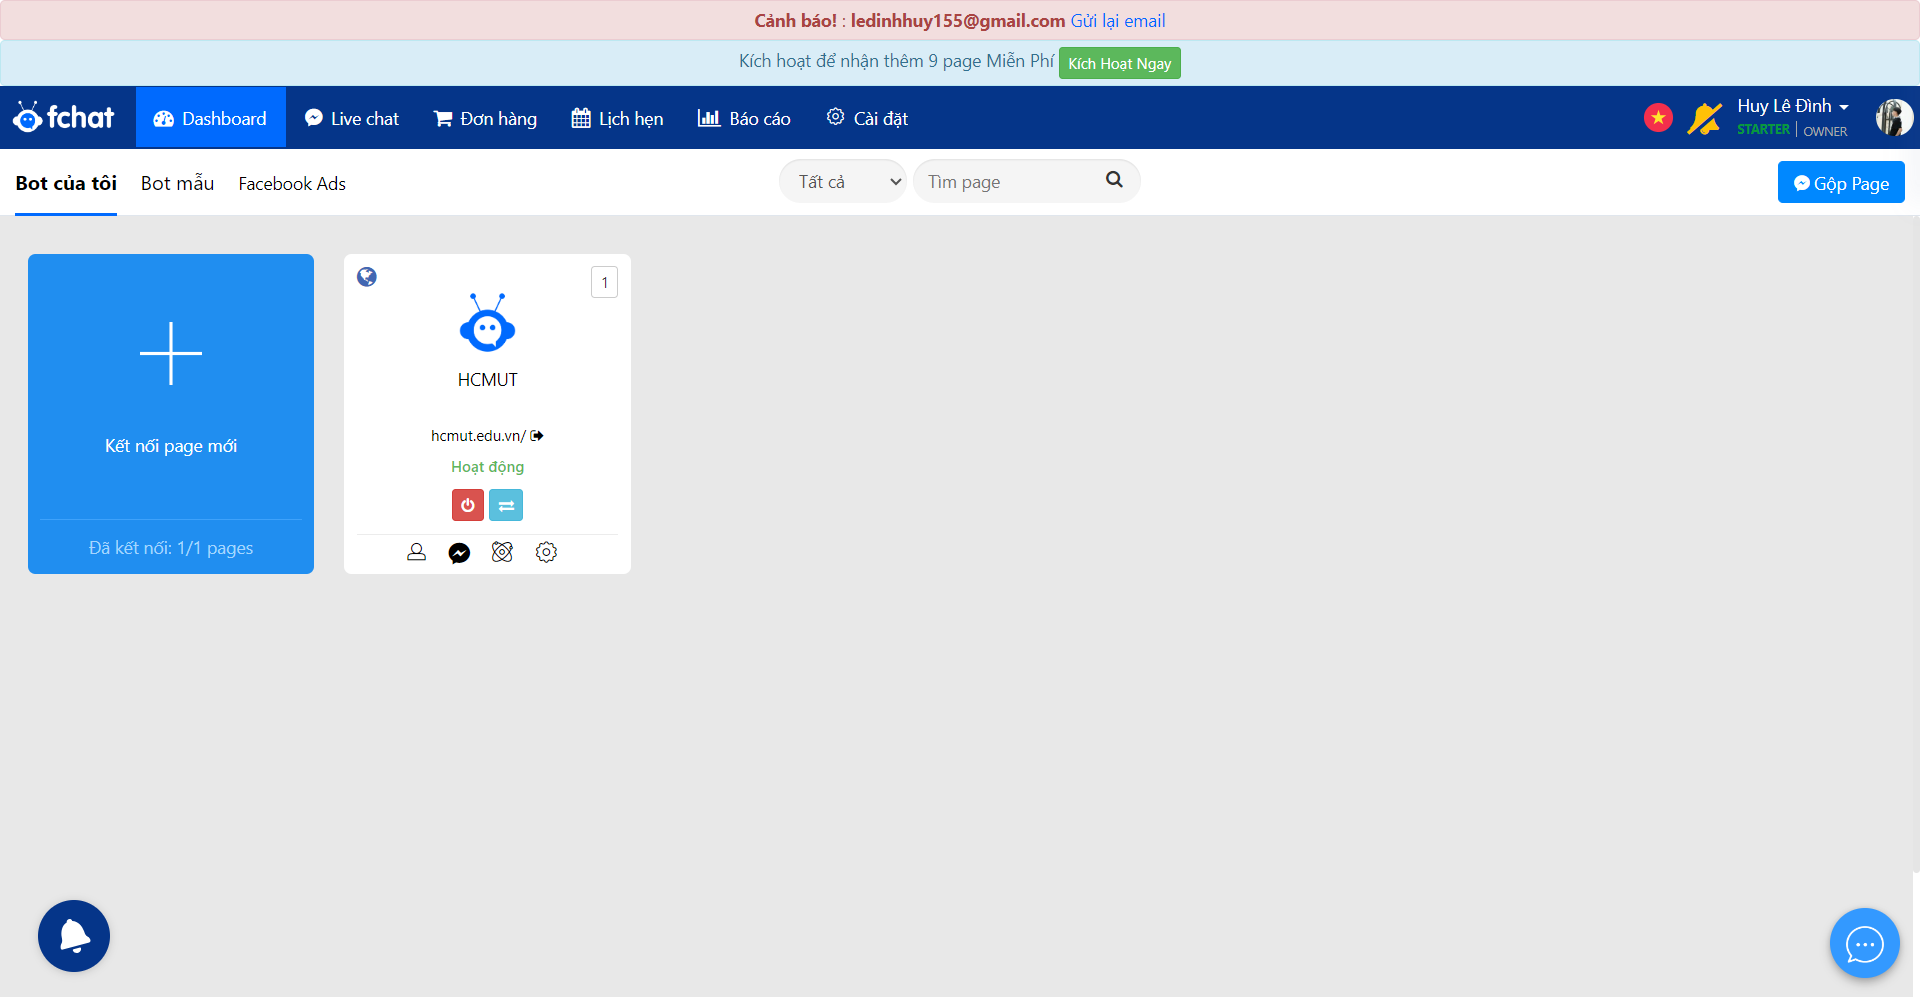
\includegraphics[width=1\linewidth]{Images/fchatdashboard.png}
    \vspace{0.5cm}
    \caption{Giao diện trang Dashboard của Fchat}
    \label{fig:enter-label}
\end{figure}
\begin{figure}[H]
    \centering
    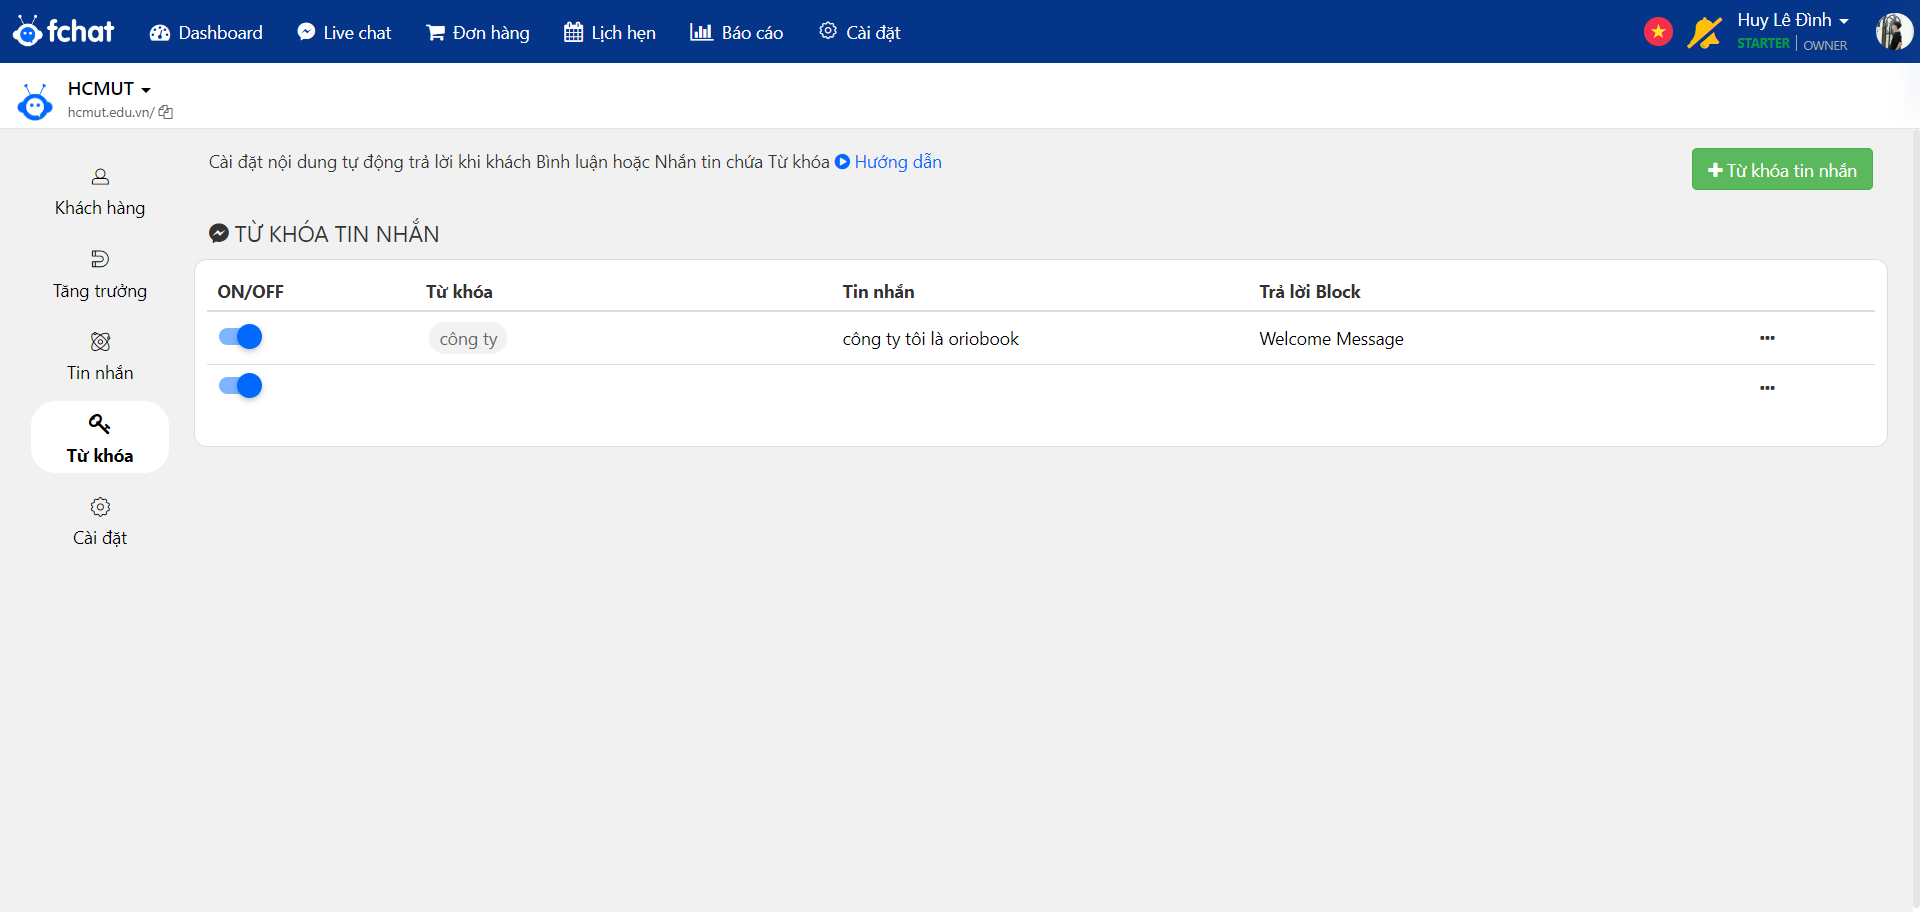
\includegraphics[width=1\linewidth]{Images/tukhoafchat.png}
    \vspace{0.5cm}
    \caption{Giao diện quản lý từ khóa tin nhắn của Fchat}
    \label{fig:enter-label}
\end{figure}
\begin{figure}[H]
    \centering
    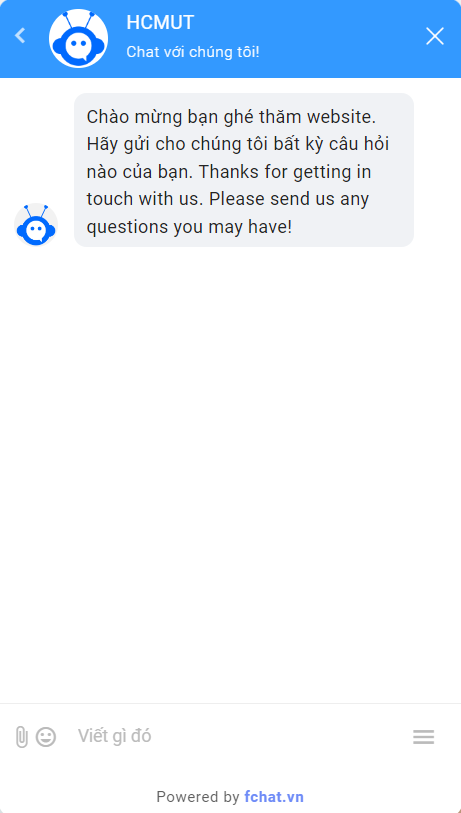
\includegraphics[width=0.5\linewidth]{Images/chatfchat.png}
    \vspace{0.5cm}
    \caption{Giao diện khung chat của Fchat}
    \label{fig:enter-label}
\end{figure}
\subsubsection{Các tính năng chính}
Fchat là một nền tảng chatbot dành cho doanh nghiệp, tập trung vào việc tự động hóa giao tiếp với khách hàng thông qua Facebook Messenger và các kênh khác. Dưới đây là các tính năng chính và mô tả về Fchat:

\begin{itemize}
    \item \textbf{Tự động trả lời tin nhắn:} Fchat cho phép thiết lập chatbot tự động trả lời các tin nhắn từ khách hàng trên Facebook Messenger, giúp doanh nghiệp phản hồi nhanh chóng và không bị gián đoạn.
    
    \item \textbf{Tự động bình luận và trả lời bình luận trên bài viết:} Chatbot Fchat có thể tự động trả lời bình luận của khách hàng trên các bài viết Facebook, đồng thời gửi tin nhắn riêng (inbox) để tiếp tục tư vấn hoặc quảng bá sản phẩm.
    \item \textbf{Gửi tin nhắn hàng loạt (Broadcasting):} Fchat hỗ trợ tính năng gửi tin nhắn hàng loạt đến nhiều khách hàng cùng lúc, giúp doanh nghiệp tiếp thị và quảng bá sản phẩm hiệu quả.

    \item \textbf{Tạo lịch hẹn và tự động nhắc nhở:} Fchat hỗ trợ chức năng tạo lịch hẹn với khách hàng ngay trong hội thoại, đồng thời gửi thông báo nhắc nhở tự động trước số ngày, số giờ tùy chỉnh.

    \item \textbf{Tạo đơn hàng tự động:} Fchat hỗ trợ doanh nghiệp tự động tạo đơn hàng khi khách hàng tương tác qua các kênh như Livestream, quảng cáo, form đặt hàng hoặc trang bán hàng (selling page). Điều này giúp quy trình bán hàng trở nên nhanh chóng và tiện lợi.

    \item \textbf{Kết nối và đồng bộ với các đơn vị vận chuyển:} Fchat có thể kết nối với các đơn vị vận chuyển như Giao Hàng Nhanh, Giao Hàng Tiết Kiệm, Viettel Post, v.v., giúp tự động đồng bộ và quản lý đơn hàng vận chuyển.
    
    \item \textbf{Thống kê và báo cáo chi tiết:} Fchat cung cấp các công cụ thống kê chi tiết về hiệu quả tương tác của chatbot, giúp doanh nghiệp nắm bắt được mức độ hiệu quả của từng chiến dịch và kịch bản.
\end{itemize}
\begin{figure}[H]
    \centering
    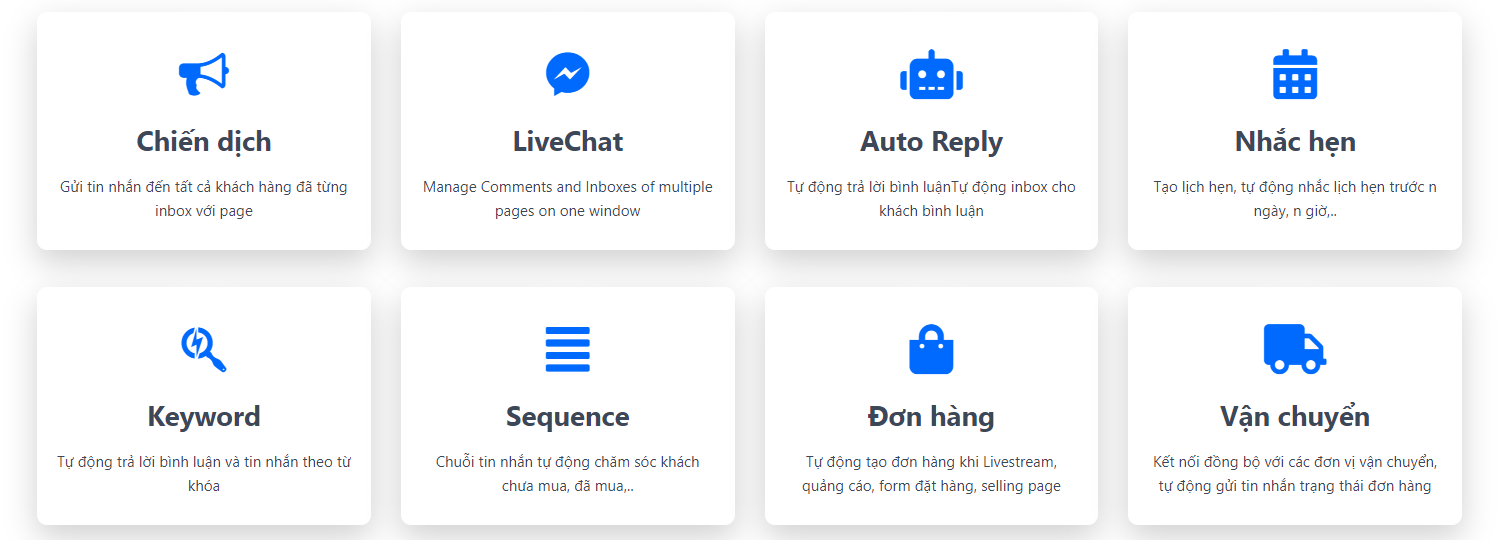
\includegraphics[width=1\linewidth]{Images/featurefchat.png}
    \vspace{0.5cm}
    \caption{Các tính năng cơ bản của Fchat}
    \label{fig:enter-label}
\end{figure}
\subsubsection{Phân tích SWOT}
\begin{table}[H]
\centering
\begin{tabular}{|p{7cm}|p{7cm}|}
\hline
 \begin{center}
     Strengths
 \end{center} & \begin{center}
     Weaknesses
 \end{center}  \\
\hline
\begin{itemize}
    \item Tích hợp tính năng hỗ trợ tự động hóa bán hàng qua Livestream.
    \item Hỗ trợ tạo lịch hẹn và tự động nhắc nhở khách hàng.
    \item Kết nối với các đơn vị vận chuyển và tự động cập nhật trạng thái đơn hàng.
    \item Nền tảng thân thiện với người dùng, dễ dàng tích hợp vào các hệ thống kinh doanh.
\end{itemize} &  
\begin{itemize}
    \item Tập trung vào Facebook Messenger, website, thiếu đa dạng kênh hỗ trợ như Instagram hoặc Zalo.
    \item Quá nhiều tính năng gây phức tạp, khó thể thành thạo trong khoảng thời gian ngắn.
\end{itemize}\\
\hline
\begin{center}
    Opportunities
\end{center} & \begin{center}
    Threats
\end{center}\\
\hline
\begin{itemize}
    \item Tiềm năng lớn trong thị trường livestream bán hàng, đặc biệt tại Việt Nam.
\item Khả năng phát triển các tính năng tích hợp cho doanh nghiệp trong lĩnh vực thương mại điện tử.
\end{itemize} &  
\begin{itemize}
    \item Các nền tảng cạnh tranh khác ngày càng hoàn thiện và cung cấp các tính năng tương tự.
\item Yêu cầu phát triển tính năng mới liên tục để đáp ứng nhu cầu người dùng.
\end{itemize}\\
\hline
\end{tabular}
\caption{Bảng phân tích SWOT cho hệ thống Fchat}
\end{table}
\subsection{TuDongChat}
\subsubsection{Giới thiệu}
TuDongChat là công cụ AI Chatbot sử dụng sức mạnh của trí tuệ nhân tạo nhằm xây dựng những tính năng tự động hàng loạt, thay thế đến 99
\% sức mạnh con người. Với công cụ này, người dùng có thể tích hợp vào bất cứ nền tảng nào như website, Facebook, Zalo một cách dễ dàng mà không cần biết về kiến thức lập trình.


Được phát triển bởi công ty Anthropic, một trong những công ty dẫn đầu về công nghệ trí tuệ nhân tạo. TuDongChat ra mắt vào tháng 6/2022 với sứ mệnh cung cấp giải pháp Chatbot tiện lợi, hiệu quả cho các doanh nghiệp. Mặc dù chỉ mới hoạt động trên thị trường được 2 năm, song phần mềm này nhanh chóng nhận được sự quan tâm của đông đảo khách hàng.

\href{https://tudongchat.com/}{Link truy cập}
\subsubsection{UI/UX}
\begin{figure}[H]
    \centering
    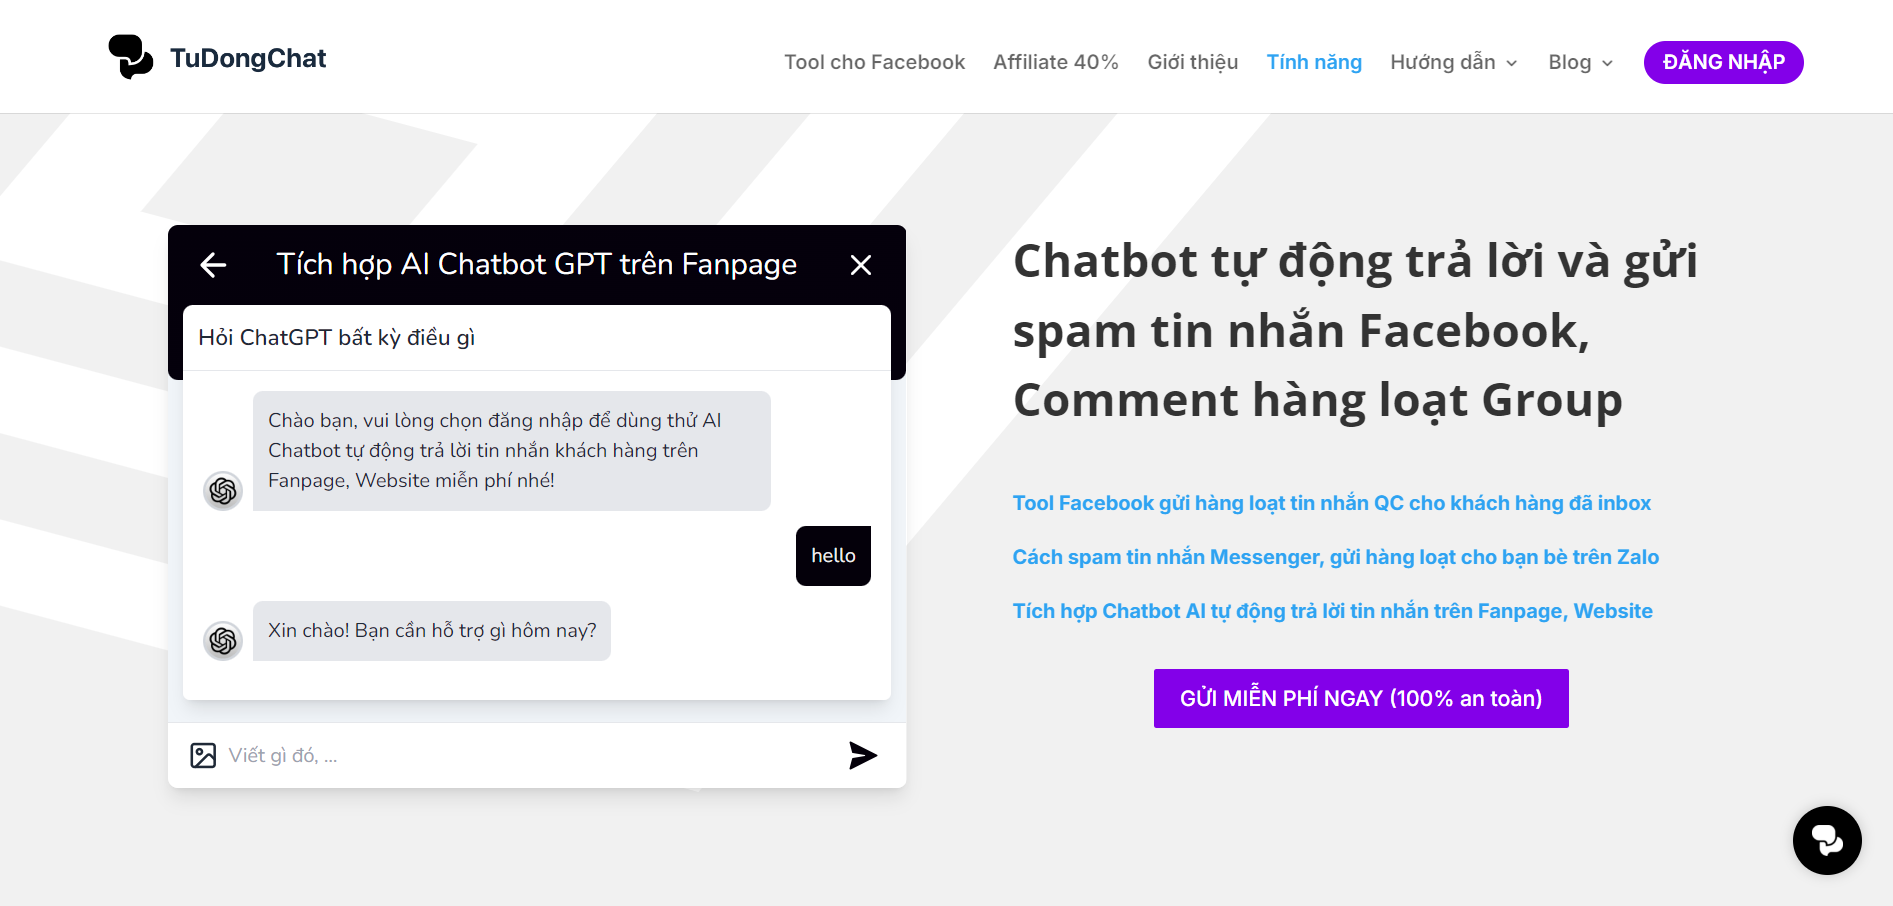
\includegraphics[width=1\linewidth]{Images/uiTuDongChat.png}
    \vspace{0.5cm}
    \caption{Giao diện trang Landing page của TuDongChat}
    \label{fig:enter-label}
\end{figure}

\begin{figure}[H]
    \centering
    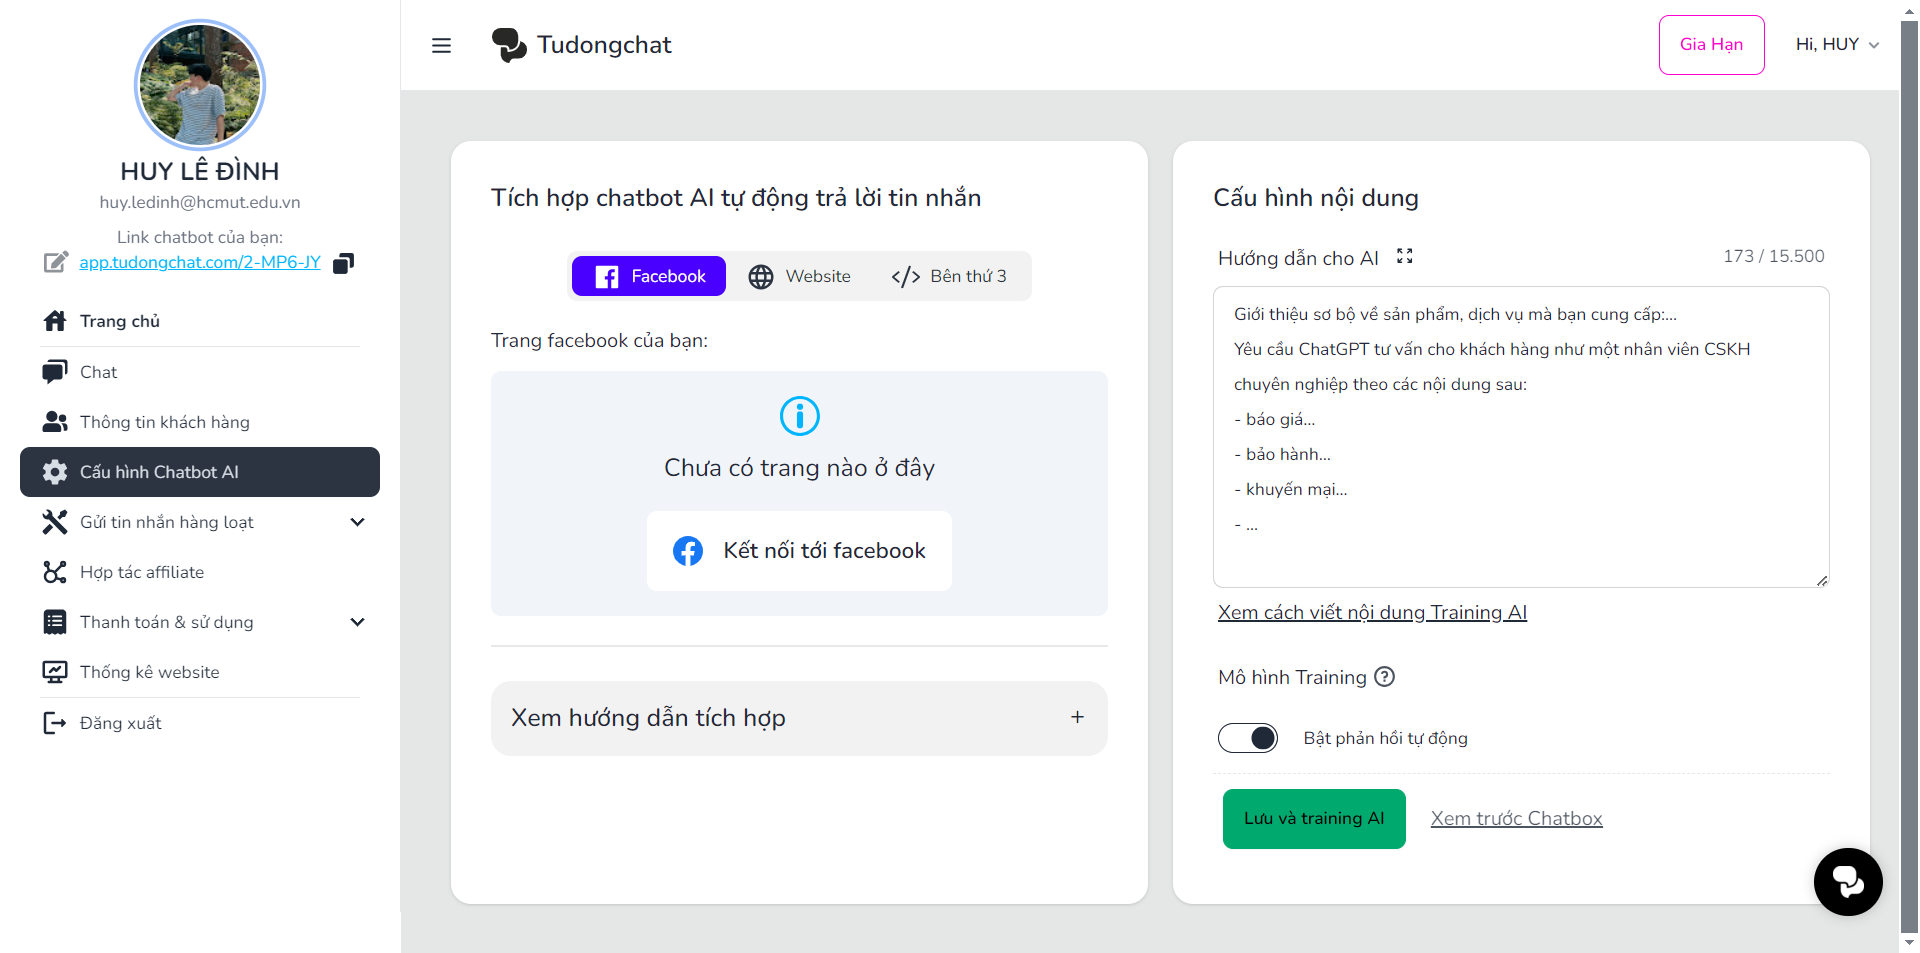
\includegraphics[width=1\linewidth]{Images/uiTuDongChat2.png}
    \vspace{0.5cm}
    \caption{Giao diện Trang chủ của TuDongChat}
    \label{fig:enter-label}
\end{figure}

\begin{figure}[H]
    \centering
    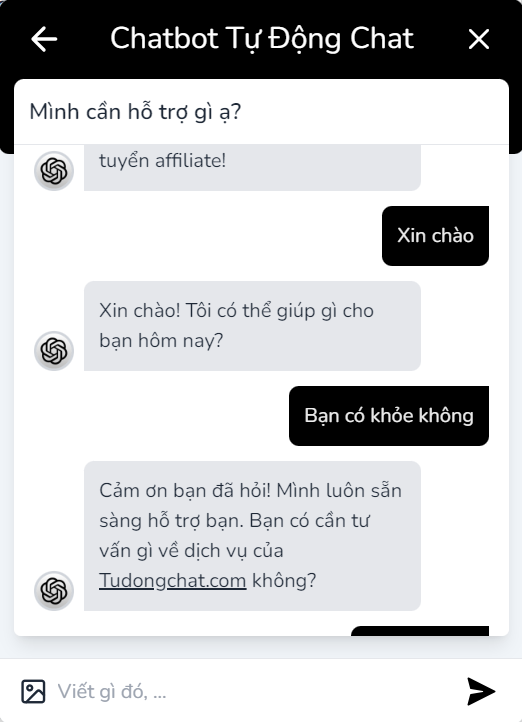
\includegraphics[width=0.5\linewidth]{Images/uiTuDongChat3.png}
    \vspace{0.5cm}
    \caption{Giao diện khung chat của TuDongChat}
    \label{fig:enter-label}
\end{figure}
\subsubsection{Các tính năng chính}
Với sức mạnh của trí tuệ nhân tạo, TuDongChat cung cấp các tính năng cơ bản sau:
\begin{itemize}
    \item \textbf{Tự động gửi tin hàng loạt:} Giúp doanh nghiệp gửi thông tin tiếp thị cho khách hàng về sản phẩm mới, chương trình khuyến mãi hoặc sự kiện sắp diễn ra. Bằng việc sử dụng trí tuệ nhân tạo để tùy biến thông điệp một cách linh hoạt, không spam, đảm bảo an toàn tuyệt đối cho tài khoản mạng xã hội Facebook \& Zalo của bạn.
    \item \textbf{Tự động tìm kiếm khách hàng tiềm năng:} AI Chatbot TuDongChat không dừng lại ở việc chờ đợi khách hàng liên hệ, mà còn tự động tham gia vào các hội nhóm Facebook, tìm kiếm các bài viết liên quan và tương tác với người dùng tiềm năng, giúp bạn mở rộng mạng lưới khách hàng một cách tự nhiên và linh hoạt.
    \item \textbf{Tự động spam comment Facebook:} AI Chatbot TuDongChat với khả năng đọc hiểu và sáng tạo nội dung theo ngữ cảnh, sẽ giúp bạn spam comment trên các hội nhóm Facebook nhưng vẫn đảm bảo an toàn 100\% cho nick Facebook của bạn.
    \item \textbf{Tự động tương tác và trả lời khách hàng một cách tự nhiên:} Cuối cùng nhưng không kém phần quan trọng, chatbot của chúng tôi không chỉ là một trợ lý cấp cao. Chúng tôi sử dụng trí tuệ nhân tạo ChatGPT để tương tác với khách hàng trên mọi nền tảng – từ website đến fanpage Facebook của bạn. Từ việc trả lời các câu hỏi cơ bản đến việc hỗ trợ mua hàng, chúng tôi đảm bảo rằng mỗi cuộc trò chuyện đều diễn ra một cách tự nhiên và đáp ứng nhanh chóng.
\end{itemize}
\begin{figure}[H]
    \centering
    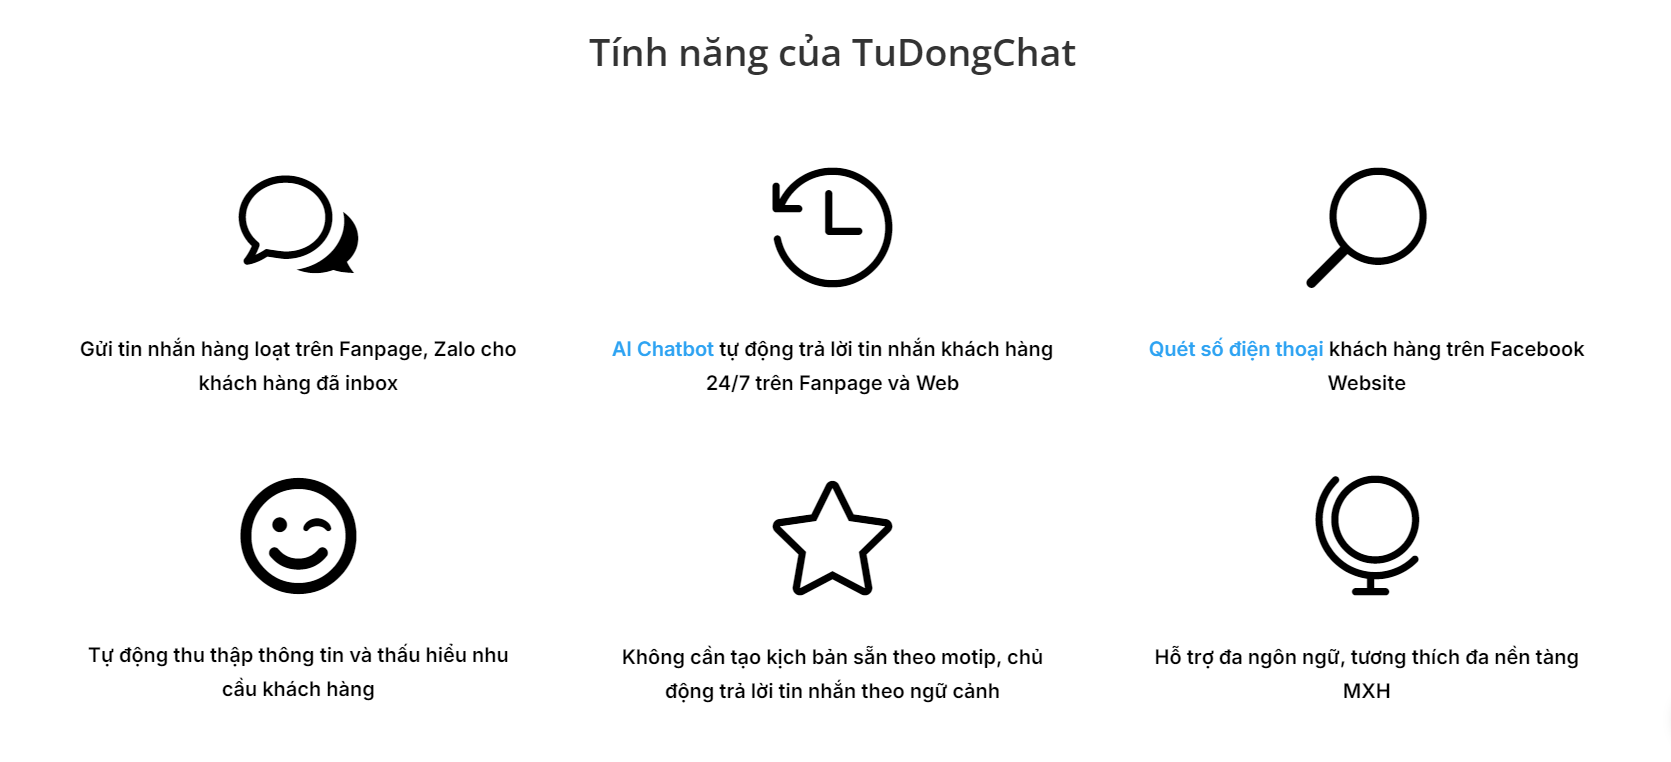
\includegraphics[width=1\linewidth]{Images/tinhnangtudongchat.png}
    \vspace{0.5cm}
    \caption{Các tính năng cơ bản của TuDongChat}
    \label{fig:enter-label}
\end{figure}
\subsubsection{Phân tích SWOT}
\begin{table}[H]
\centering
\begin{tabular}{|p{7cm}|p{7cm}|}
\hline
\begin{center}
    Strengths
\end{center}
  &  \begin{center}
      Weaknesses
  \end{center} \\
\hline
\begin{itemize}
    \item Hỗ trợ tạo chatbot tự động cho doanh nghiệp mà không yêu cầu kỹ năng lập trình.
\item Tính năng tích hợp đa kênh từ Facebook Messenger, Zalo đến website.
\item Giao diện quản lý đơn giản và tập trung vào tự động hóa các tác vụ liên quan đến chăm sóc khách hàng.

\end{itemize} &  
\begin{itemize}
    \item Tính năng chưa đa dạng bằng các nền tảng lớn khác, hạn chế trong việc tùy chỉnh các kịch bản phức tạp.
\item Thiếu các công cụ phân tích sâu sắc để theo dõi hành vi khách hàng và hiệu quả chatbot.
\end{itemize}\\
\hline
\begin{center}
    Opportunities
\end{center} & \begin{center}
    Threats
\end{center}\\
\hline
\begin{itemize}
    \item Tăng trưởng của thị trường chatbot tại Việt Nam, đặc biệt trong các ngành bán lẻ và dịch vụ.
\item Cơ hội phát triển và mở rộng thêm tính năng tự động hóa nâng cao và tích hợp với nhiều nền tảng khác.
\end{itemize} &  
\begin{itemize}
    \item Sự xuất hiện của các đối thủ cạnh tranh lớn trong nước và quốc tế với nhiều tính năng hơn.
\item Công nghệ phát triển nhanh chóng đòi hỏi liên tục đổi mới để theo kịp xu hướng.
\end{itemize}\\
\hline
\end{tabular}
\caption{Bảng phân tích SWOT cho hệ thống TuDongChat}
\end{table}